\documentclass[11pt,aspectratio=169]{beamer}
\usepackage[T1]{fontenc}
\usepackage{lmodern}
\usepackage{graphicx}
\usepackage{amsmath,amssymb,mathtools}
\usepackage{booktabs}
\usepackage{array}

\setbeamertemplate{navigation symbols}{}
\setbeamertemplate{itemize items}[circle]
\setbeamertemplate{footline}[frame number]

\title{Where We Sit: The Credit-Mediated Transition into Family-Sized Ownership}
\date{}

\begin{document}

\maketitle

% ====================================================================
\begin{frame}{The Mechanism: Credit $\to$ Ownership $\to$ Space $\to$ Child}
\small

Hacamo (2021, \emph{RFS}) identifies a causal chain in the data:
\[
\text{credit access} \;\to\; \underbrace{\text{cross DP threshold}}_{b \,\geq\, (1-\phi)\,p_i\,H_k} \;\to\; \text{ownership of a larger unit} \;\to\; \text{child}
\]

\smallskip
The killer test (his Table~8). He splits the joint outcome $\mathbf{1}\{\text{buy} \cap \text{newborn}\}$ by the size of the purchased home:

\smallskip
\centering
\begin{tabular}{lcc}
\toprule
$y = \mathbf{1}\{\text{Mortgage \& newborn \& [size]}\}$ & \textbf{Large} (4+ rooms) & \textbf{Small} ($<$4 rooms)\\
\midrule
APL $\times$ Post $\times$ Fraction OCC & $0.05$ to $0.06^{**}$ & $0.01$ (n.s.)\\
\bottomrule
\end{tabular}

\smallskip\flushleft
The credit-deregulation effect on babies works \emph{only} through purchases of bigger homes. The chain is not generic; it is the family-space chain. Supplemental tests reject income growth and housing-wealth growth as alternatives.

\end{frame}

% ====================================================================
\begin{frame}{Families Need Big Units --- Two Views}
\small

\begin{columns}[T,onlytextwidth]
\begin{column}{0.49\textwidth}
\centering
\includegraphics[width=\linewidth,height=0.62\textheight,keepaspectratio]{../code/data/ahs_supply_snapshot/output_ahs_family_unit_menu_national/ahs_bedroom_menu_by_children.png}

\smallskip
\footnotesize \emph{Within each household type:} of households with kids, $79\%$ live in 3+ bedroom units; of childless, $59\%$.
\end{column}
\begin{column}{0.49\textwidth}
\centering
\includegraphics[width=\linewidth,height=0.62\textheight,keepaspectratio]{../code/data/ahs_supply_snapshot/output_ahs_family_unit_menu_national/ahs_bedroom_share_within_size.png}

\smallskip
\footnotesize \emph{Within each size bin:} share occupied by parents rises monotonically from $6\%$ (0--1 bed) to $41\%$ (4+ bed).
\end{column}
\end{columns}

\medskip
\flushleft
Two sides of the same fact, same data: families need bigger units, and the bigger-unit stock is dominated by families. The gradient on the right ($6 \to 21 \to 29 \to 41\%$ parents) is the cleanest expression --- it says directly who occupies the family-sized stock. Source: AHS 2023.

\end{frame}

% ====================================================================
\begin{frame}{Big Units Are Owned --- Renting Is Not a Substitute}
\small

\begin{columns}[T,onlytextwidth]
\begin{column}{0.49\textwidth}
\centering
\includegraphics[width=\linewidth,height=0.62\textheight,keepaspectratio]{../code/data/ahs_supply_snapshot/output_ahs_family_unit_menu_national/ahs_bedroom_menu_by_tenure.png}

\smallskip
\footnotesize \emph{Within tenure:} of owners, $81\%$ live in 3+ bedroom units; of renters, $30\%$.
\end{column}
\begin{column}{0.49\textwidth}
\centering
\includegraphics[width=\linewidth,height=0.62\textheight,keepaspectratio]{../code/data/ahs_supply_snapshot/output_ahs_family_unit_menu_national/ahs_tenure_share_within_size.png}

\smallskip
\footnotesize \emph{Within size bin:} owner share of occupied units rises $13 \to 39 \to 75 \to 87\%$ as bedrooms grow. Renter share falls $74 \to 50 \to 19 \to 9\%$.
\end{column}
\end{columns}

\medskip
\flushleft
The within-size view (right) is the cleanest version: of all 4+ bedroom homes, $87\%$ are owner-occupied. The family-sized stock is essentially the owner-occupied stock. Reaching the family-sized margin requires owning, not paying more rent --- the structural asymmetry our model captures via $\max H_k > \bar h_R$. Source: AHS 2023.

\end{frame}

% ====================================================================
\begin{frame}{Across Metros: Where Family-Sized Stock Diverges, So Does Fertility}
\small

\begin{columns}[T,onlytextwidth]
\begin{column}{0.49\textwidth}
\centering
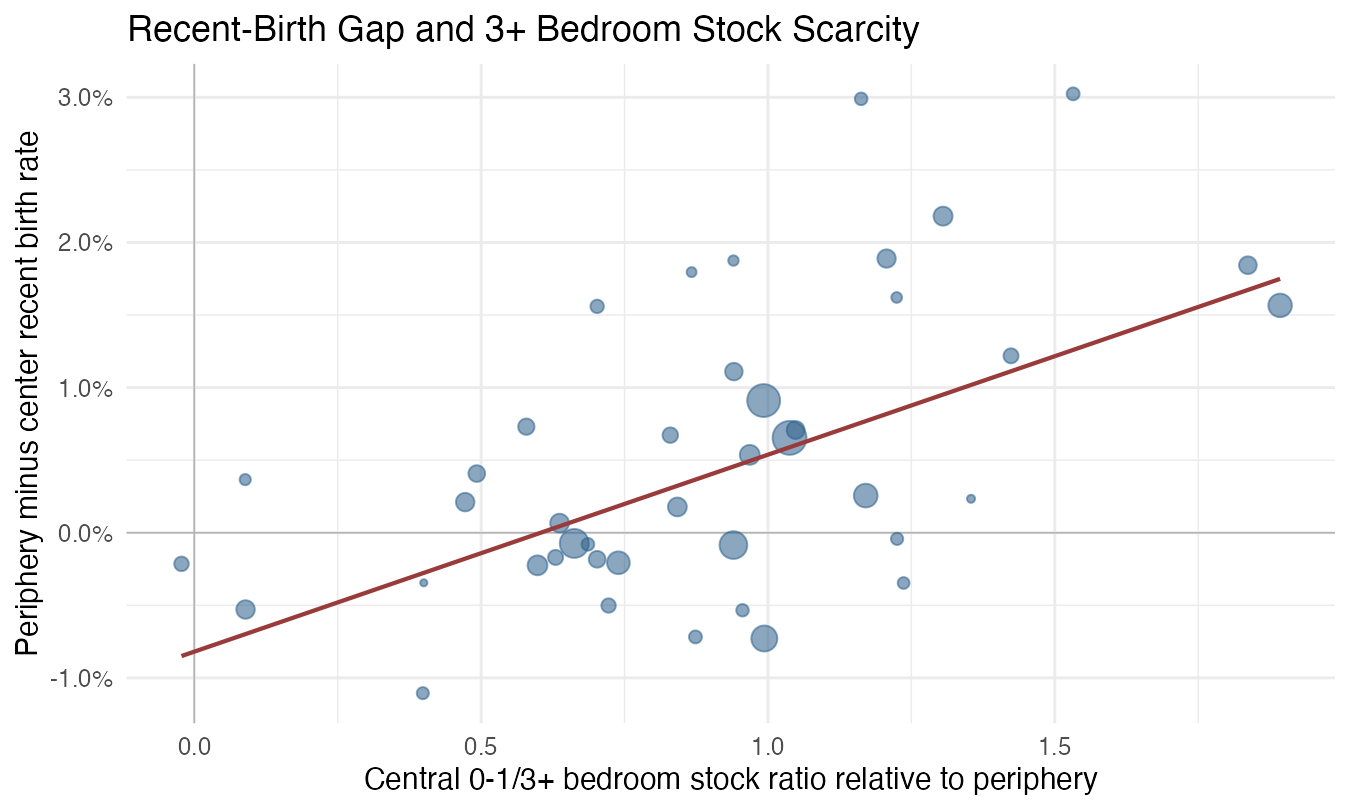
\includegraphics[width=\linewidth,height=0.58\textheight,keepaspectratio]{../docs/model/family_space_empirical_packet_2026-05-24/figures/original_recent_birth_gap_vs_stock_scarcity.png}

\smallskip
\footnotesize Periphery--center \emph{recent-birth gap} rises with central 3+ bedroom stock scarcity.
\end{column}
\begin{column}{0.49\textwidth}
\centering
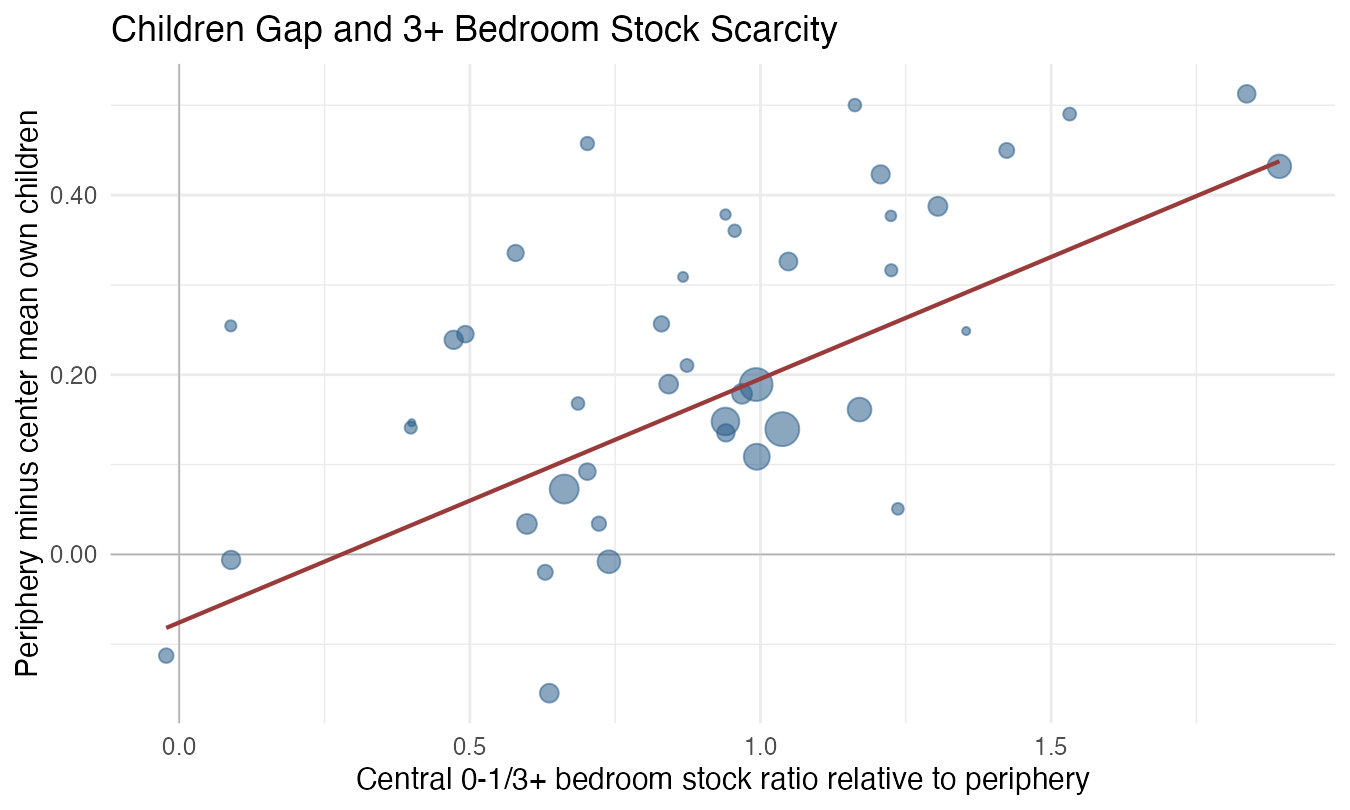
\includegraphics[width=\linewidth,height=0.58\textheight,keepaspectratio]{../docs/model/family_space_empirical_packet_2026-05-24/figures/original_mean_children_gap_vs_stock_scarcity.png}

\smallskip
\footnotesize Periphery--center \emph{mean own children gap} rises with the same scarcity measure.
\end{column}
\end{columns}

\medskip
\flushleft
\footnotesize
ACS 2012--2023, 42 large MMS metros. $x$-axis: log of the central $\frac{0\text{--}1\,\text{bed}}{3\text{+}\,\text{bed}}$ stock ratio relative to periphery (higher $=$ central family-sized stock is scarcer, Couillard-style measure). $y$-axes: periphery $-$ center on the row's outcome.

\smallskip
The same axis predicts \emph{parent centrality gap} with slope $0.147$ (SE $0.026$, $p < 10^{-6}$). Robust to expanding the sample to 80 metros (top-100-c25).

\end{frame}

% ====================================================================
\begin{frame}{Same Pattern, Cleanest Availability Measure: Share of Family-Sized Stock}
\small

\centering
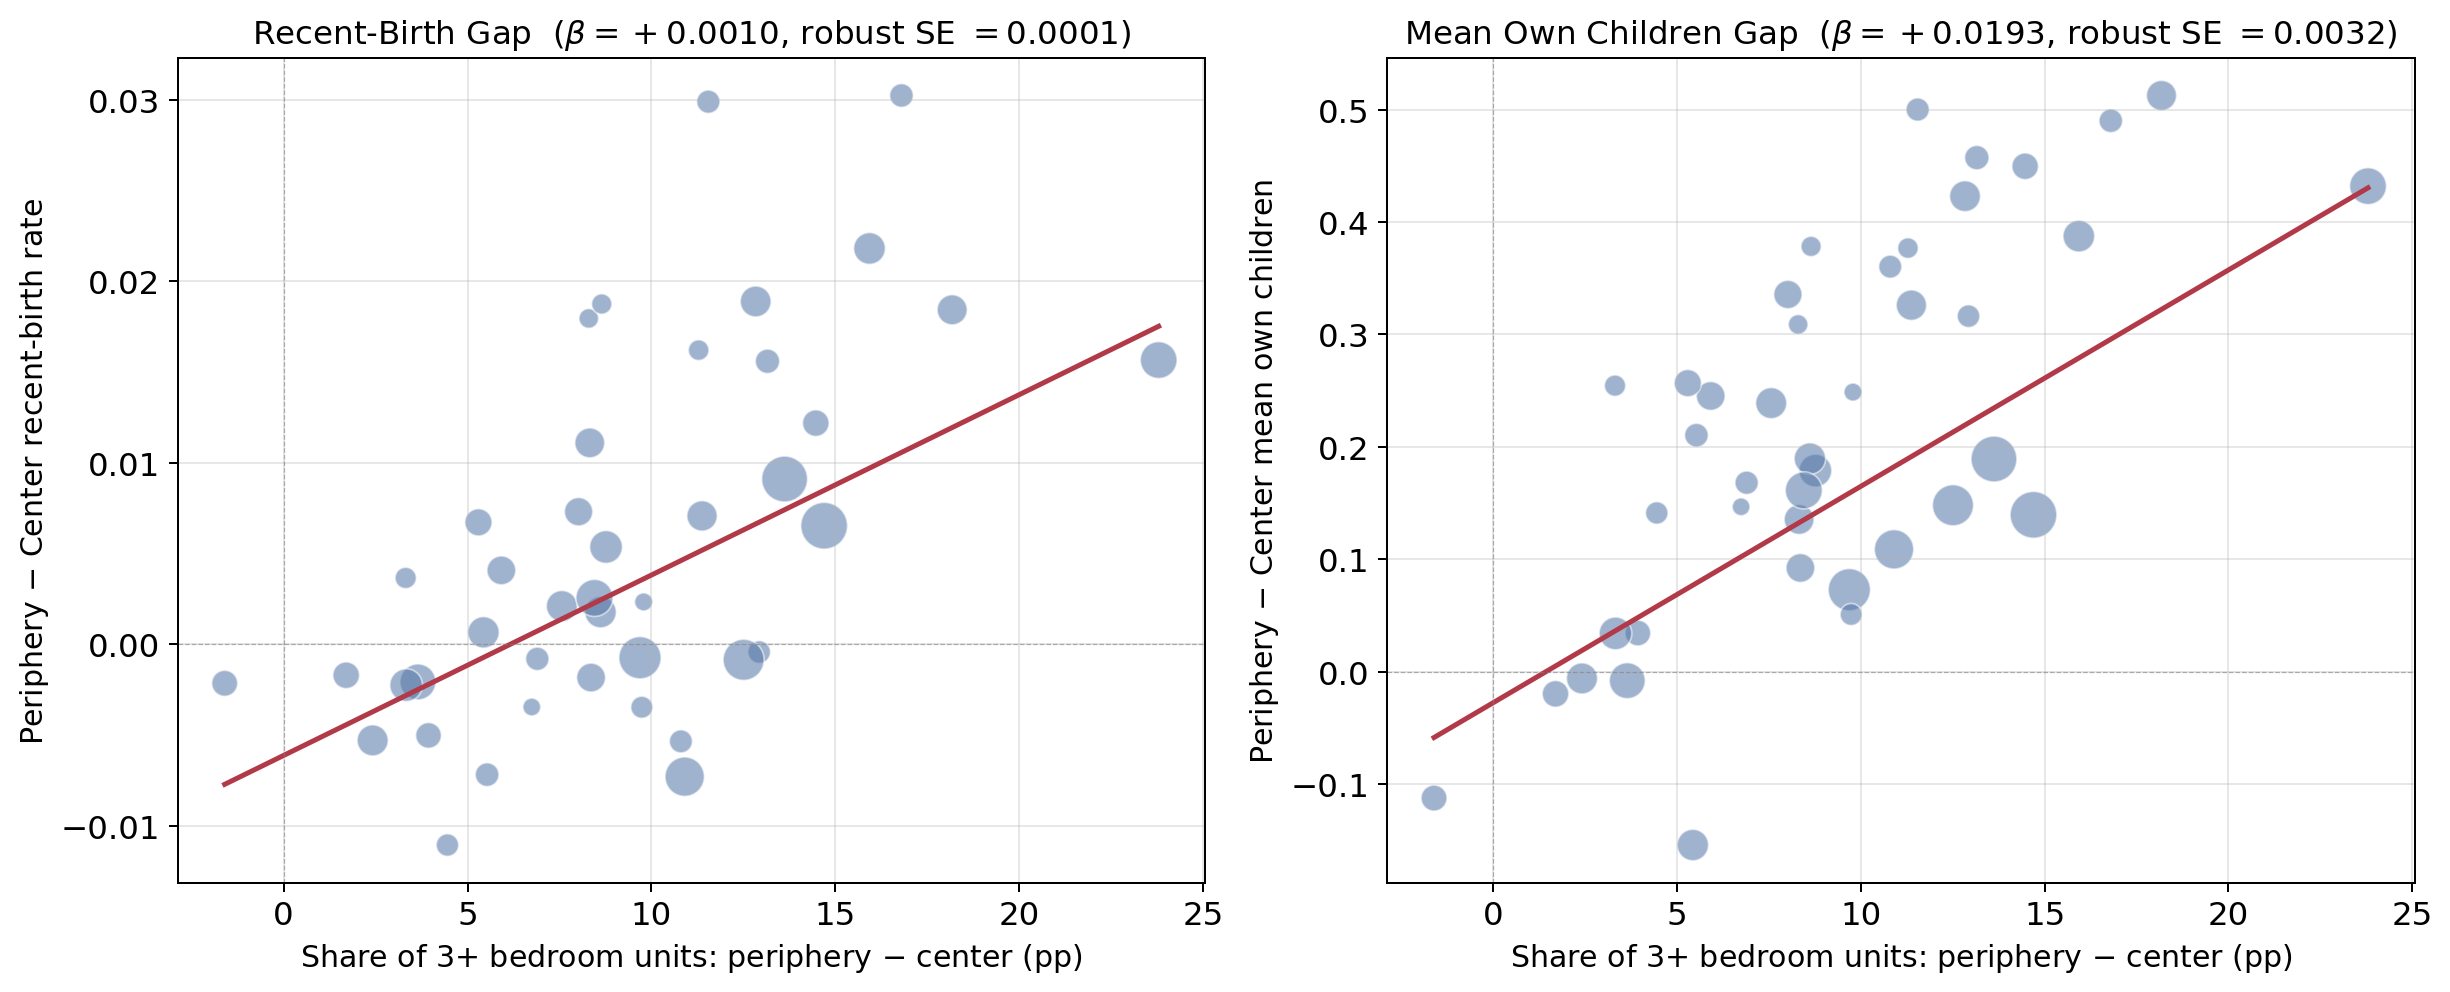
\includegraphics[width=0.95\textwidth,height=0.62\textheight,keepaspectratio]{../docs/model/family_space_empirical_packet_2026-05-24/figures/family_share_gap_vs_fertility_gap.png}

\medskip
\flushleft
\footnotesize
ACS 2012--2023, 42 large MMS metros. $x$-axis: \emph{share of $3{+}$ bedroom units in periphery $-$ share in center}, in percentage points (mean $9.2$, range $-1.6$ to $23.8$). $y$-axes: periphery $-$ center on the row's outcome.

\smallskip
Each $+1$ pp in the family-stock share gap is associated with $\sim$$0.1$ pp on the recent-birth gap and $0.02$ on the mean-children gap (both robust SE small enough to clear conventional thresholds). The mean-rooms-gap and bedroom-scarcity log-ratio versions give the same picture in different units.

\end{frame}

% ====================================================================
\begin{frame}{Our PSID: Families Space Out at Birth}
\small

The destination side of Hacamo's chain shows up cleanly in PSID. Event study around first birth, rooms as outcome:

\smallskip
\centering
\begin{tabular}{lcc}
\toprule
& \textbf{First birth} & \textbf{Second birth}\\
\midrule
Pre-event mean (rooms) & $6.01$ & $6.14$\\
$\alpha_{+3}$ (rooms at +3 yrs) & $\mathbf{+0.66}\,(\text{SE } 0.15)$ & $\mathbf{+0.70}\,(\text{SE } 0.18)$\\
$\alpha_{+5}$ (rooms at +5 yrs) & $+0.84\,(0.15)$ & $+0.72\,(0.18)$\\
$N$ obs / IDs & $248{,}566\,/\,23{,}041$ & $155{,}358\,/\,15{,}568$\\
\bottomrule
\end{tabular}

\smallskip\flushleft
Both first and second births add roughly $0.7$ rooms by year $+3$. Babies arrive with bigger homes. Combined with Hacamo's Table~8 and the AHS asymmetry, the chain is end-to-end: families need big units, big units are owned, getting them requires the credit-mediated transition.

\end{frame}

% ====================================================================
\begin{frame}{The Wealth Gate: Renters Who Can't Clear the DP Stay Childless}
\small

Among PSID renters at ages 25--30, pre-first-birth ($N = 2{,}961$, followed to age 45). Define DP shortfall at the FHA $3.5\%$ floor:
\[
\text{shortfall}_i \;=\; \mathbf{1}\!\left\{ \text{liquid wealth}_i \;<\; 0.035 \cdot P^{\text{target}}_t \right\}.
\]

\medskip
\begin{columns}[T,onlytextwidth]
\begin{column}{0.50\textwidth}
\centering
\begin{tabular}{lr}
\toprule
& Shortfall rate \\
\midrule
Bottom income tercile & $90\%$ \\
Middle income tercile & $83\%$ \\
Top income tercile    & $84\%$ \\
\bottomrule
\end{tabular}

\smallskip
\footnotesize
$90\%$ of low-income young renters lack the cash for a $3.5\%$ FHA down payment on a typical first home. Even most top-income young renters fall short.
\end{column}
\begin{column}{0.50\textwidth}
\centering
\begin{tabular}{lrrr}
\toprule
$y =$ childless by 45 & $\hat\beta$ & SE & $p$ \\
\midrule
Shortfall                          & $\mathbf{0.088}$ & $0.029$ & $0.003$ \\
\quad + $\log$ income              & $0.088$          & $0.029$ & $0.003$ \\
\quad + $\log$ income + $\log$ NW  & $0.088$          & $0.029$ & $0.003$ \\
\bottomrule
\end{tabular}

\smallskip
\footnotesize
DP-short renters are $8.8$ pp more likely to remain childless by $45$, controlling for log income and log wealth. The DP gate predicts fertility, not the income level alone.
\end{column}
\end{columns}

\medskip
\centering
\footnotesize PSID $1984$--$2019$. $P^{\text{target}}_t$ = median first-time-buyer home value in same year-bin.

\end{frame}

% ====================================================================
\begin{frame}{Existing Models Miss the Credit-Mediated Entry; Our Model Has It}
\small

\centering
\begin{tabular}{p{0.22\textwidth}p{0.23\textwidth}p{0.23\textwidth}p{0.23\textwidth}}
\toprule
 & \textbf{Couillard (2025)} & \textbf{Cumming \& Dettling (2024)} & \textbf{Our model}\\
\midrule
Tenure regime & owner / renter as states & owners only (existing mortgage holders) & owner / renter as states \\
\addlinespace
Family-sized unit margin & bedrooms 1, 2, 3+ & not modeled & discrete owner sizes $H_k$ with $\max H_k > \bar h_R$ \\
\addlinespace
Credit / DP constraint & \textbf{absent}: no $\phi$, no house prices, no liquid wealth state & not modeled; uses ARM/FRM payment shocks instead & $b \geq (1-\phi)\,p_i\,H_k$ with $\phi = 0.80$ (DUE standard) \\
\addlinespace
What an APL/OCC credit shock would do & no model object responds & changes monthly payment, not the rent-to-own transition & relaxes the threshold; marginal renters cross into a larger $H_k$ \\
\bottomrule
\end{tabular}

\smallskip\flushleft
Couillard can describe the destination but not the credit trigger that lets a marginal renter reach it. Cumming \& Dettling identify a real fertility response to mortgage credit but on the post-ownership cash-flow margin, not the entry margin. We are the only structural framework where Hacamo's specific causal chain has a model object behind every arrow.

\end{frame}

% ====================================================================
\begin{frame}{What This Buys}
\small

Three structural ingredients deliver the Hacamo chain:
\begin{enumerate}
\item Discrete tenure choice --- rent or own as distinct regimes.
\item Collateral constraint $b \geq (1-\phi)\,p_i\,H_k$, $\phi = 0.80$ following DUE.
\item Tenure-asymmetric housing services: $\max H_k > \bar h_R$, so the family-sized units AHS shows in the data are reachable only through ownership.
\end{enumerate}

\medskip
What this lets us do that Couillard's framework cannot:
\begin{itemize}
\item Structural quantification of Hacamo's reduced-form chain. The fertility response to a credit shock has an explicit decomposition into DP-threshold crossings and post-crossing housing-size choices.
\item A credit-side counterfactual portfolio: DP relief ($\phi \uparrow$), FHA-style threshold expansion, parent-targeted credit subsidies. These pull a lever Couillard's supply-only model does not have.
\item A natural connection to the spatial dimension: $p_i$ varies across center and periphery, so the credit gate binds differently across locations and ties cleanly into the parent-vs-non-parent sorting fact in MMS.
\end{itemize}

\end{frame}

\end{document}
